\documentclass[tikz,border=10pt]{standalone}
\usepackage{amsmath}
\begin{document}
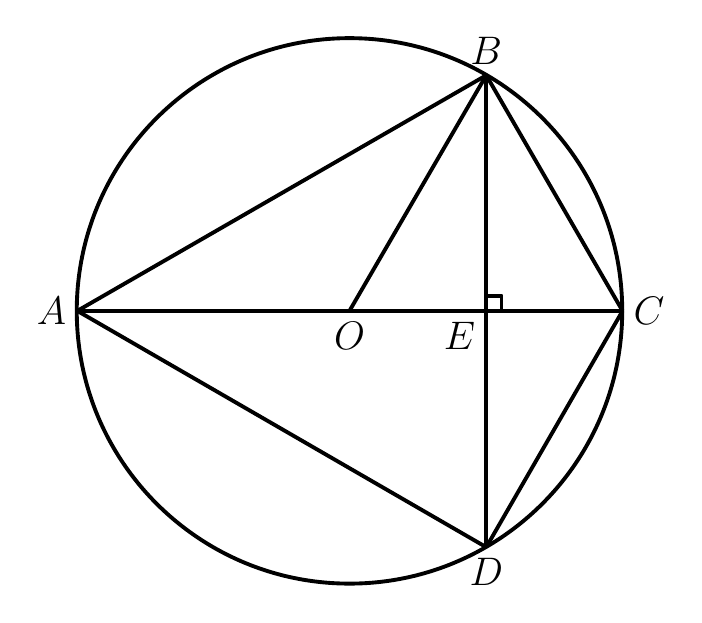
\begin{tikzpicture}[line width=1.4pt, line join=round]
% Coordinates: origin at O, scale s = 0.017621 cm per px, y flipped
\coordinate (O) at (0,0);
\coordinate (A) at (-3.4566,0);
\coordinate (C) at (3.4681,0);
\coordinate (B) at (1.737,2.992);
\coordinate (D) at (1.737,-3.001);
\coordinate (E) at (1.737,0);

% Circle centred at O, radius 196.56 px
\draw (O) circle (3.4637);

% Segments (solid), ending exactly at vertices
\draw (A) -- (C);
\draw (A) -- (B);
\draw (A) -- (D);
\draw (B) -- (C);
\draw (C) -- (D);
\draw (B) -- (D);
\draw (B) -- (O);

% Right-angle mark at E (arms along AC and BD), side about 11 px
\draw (1.931,0) -- (1.931,0.194) -- (1.737,0.194);

% Labels
\node[left, font=\fontsize{14.5}{17.4}\selectfont] at (A) {$A$};
\node[above, font=\fontsize{14.5}{17.4}\selectfont] at (B) {$B$};
\node[right, font=\fontsize{14.5}{17.4}\selectfont] at (C) {$C$};
\node[below, font=\fontsize{14.5}{17.4}\selectfont] at (D) {$D$};
\node[below, font=\fontsize{14.5}{17.4}\selectfont] at (O) {$O$};
\node[below left, font=\fontsize{14.5}{17.4}\selectfont] at (E) {$E$};
\end{tikzpicture}
\end{document}